\documentclass[aspectratio=169]{beamer}

% because we need to claim weird things
\newtheorem{claim}{Claim}
\newtheorem{defn}{Definition}
%\newtheorem{lemma}{Lemma}
\newtheorem{thm}{Theorem}
\newtheorem{vita}{Vit\ae}
\newtheorem{qotd}{Quote of the Day}

\usepackage{algorithm}
\usepackage{algpseudocode}
\usepackage{listings}
\usepackage{color}
\usepackage{graphics}
\usepackage{ulem}
\bibliographystyle{unsrt}

% background image
\usebackgroundtemplate%
{%
    
\includegraphics[width=\paperwidth,height=\paperheight]{../artifacts/stemulus.pdf}%
}
\setbeamertemplate{caption}[numbered]
\lstset{%
	breaklines=true,
	captionpos=b,
	frame=single,
	keepspaces=true,
	showstringspaces=false
}

% page numbers
\addtobeamertemplate{navigation symbols}{}{%
    \usebeamerfont{footline}%
    \usebeamercolor[fg]{footline}%
    \hspace{1em}%
    \insertframenumber/\inserttotalframenumber
}

% presentation header
\usetheme{Warsaw}
\title{Regular Expressions}
\author{Dylan Lane McDonald}
\institute{CNM STEMulus Center\\Web Development with PHP}
\date{\today}

\begin{document}
\lstset{language=PHP}
\begin{frame}
\titlepage
\end{frame}

\begin{frame}
\frametitle{Outline}
\tableofcontents
\end{frame}

\section{Introduction to Regular Expressions}
\subsection{Theoretical Foundations}
\begin{frame}
\frametitle{What are Regular Expressions?}
\begin{defn}
A \textbf{regular expression} is a pattern that represents all the possible permutations of a string.
\end{defn}
\pause
Think of a regular expression as a plan for how strings should look. Informally, a regular expression for a US ZIP code would be, ``Five digits, optionally followed by a dash and four digits.'' The regular expression doesn't name all the possible ZIP codes, but gives an acceptance test as to whether a given string is a valid ZIP code. For instance:
\begin{itemize}
	\item 87102: \textbf{Pass}
	\item 87102-3516: \textbf{Pass}
	\item 871023516: \textbf{Fail}
	\item 8710: \textbf{Fail}
\end{itemize}
\end{frame}

\begin{frame}
\frametitle{Formalizing Regular Expressions}
Regular expressions fundamentally work with strings, whose atomic unit is a \textbf{character}. The set of all possible characters in a string is known as an \textbf{alphabet}, denoted by the Greek letter $\Sigma$. Regular expressions have three basic operations on alphabets:
\begin{itemize}
	\item \textbf{Separation}: the Boolean \textbf{OR}, ``either this character or that character''
	\item \textbf{Quantification}: The number of characters expected in this part of the string (e.g., ``3 or more digits'')
	\item \textbf{Grouping}: denoted by parentheses, characters in an alphabet are grouped to define the scope and precedence of separation of quantification
\end{itemize}
A regular expression is simply a sequence of one or more of the preceding operations.
\end{frame}

\subsection{Finite State Machines}
\begin{frame}
\frametitle{Further Formalizing Regular Expressions}
Take an informal regular expression for allowable file names: ``Start with an alphabetic character, optionally followed by 0 or more alphanumeric characters, followed by 1 dot, followed by two or three alphabetic characters.'' \pause Notice we have three alphabets:
\begin{enumerate}
	\item $\Sigma_\alpha = \{a, b, c, \dots, z\}$ (alphabetic)
	\item $\Sigma_\delta = \{0, 1, 2, \dots, 9\}$ (numeric)
	\item $\Sigma_. = \{ . \}$ (dot)
\end{enumerate}
\pause
Let * denote ``0 or more'' and ? denote ``0 or 1.'' Now, we can denote this regular expression as:
\[\alpha\left[\alpha \mid \delta \right]^* . \alpha^2 \alpha^?\]
Internally, the regular expression engine creates a finite state machine, as depicted in Figure \ref{fig:dfa}.
\end{frame}

\begin{frame}
\frametitle{Finite State Machine}
The finite state machine is basically a formal map of how strings are formed. If the string can arrive at the terminal states $q_5$ or $q_6$, we say the string \textbf{passes} the regular expression. Otherwise, it gets stuck in the finite state machine and \textbf{fails}.
\begin{figure}
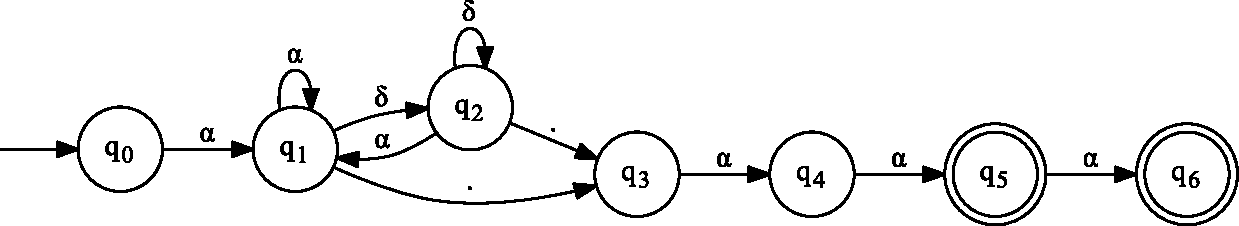
\includegraphics[scale=0.55]{../artifacts/regexp-dfa.pdf}
\caption{Finite State Machine}
\label{fig:dfa}
\end{figure}
All regular expressions can be expressed as finite state machines and all deterministic finite state machines can be expressed as regular expressions.
\end{frame}

\section{Using Regular Expressions}
\subsection{Common Syntax}
\begin{frame}
\frametitle{Character Classes \& Operators}
Regular expressions come in two major flavors: Perl Compatible Regular Expressions (PCREs) and POSIX. PHP and JavaScript use PCRE syntax.\footnote{PHP has deprecated functions for POSIX regular expressions.} This is a partial list. Use a cheat sheet! \cite{cheatography}
\begin{table}
\begin{tabular}{|l|l|l|l|}
\hline
\textbf{Item} & \textbf{Comment} & \textbf{Item} & \textbf{Comment}\\
\hline
\texttt{.} (dot) & matches \textbf{any} character & \texttt{\textbackslash s} & Whitespaces \texttt{[ \textbackslash t\textbackslash r\textbackslash n\textbackslash v]}\\
\hline
\texttt{\$} & end of line & \texttt{*} & Zero or more\\
\hline
\texttt{\textasciicircum} & beginning of line & \texttt{?} & Zero or one\\
\hline
\texttt{[abc]} & Characters a, b, or c & \texttt{+} & One or more\\
\hline
\texttt{\textbackslash d} & Digits \texttt{[0-9]} & \texttt{\{$m$,$n$\}} & $m$ or more, no more than $n$\\
\hline
\end{tabular}
\caption{Common Regular Expression Commands}
\end{table}
\end{frame}

\subsection{JavaScript}
\begin{frame}[fragile]
\frametitle{JavaScript Regular Expressions}
\begin{lstlisting}[caption=JavaScript Regular Expression Example,label=lis:javascript]
var regex = /^[a-z][\da-z]*\.[a-z]{2}[a-z]?$/;
var passed = regex.test("foo.js");
if(passed === true) {
  console.log("Regular expression passed");
} else {
  console.log("Regular expression failed");
}
\end{lstlisting}
\end{frame}

\subsection{PHP}
\begin{frame}[fragile]
\frametitle{PHP Regular Expressions}
\begin{lstlisting}[caption=PHP Regular Expression Example,label=lis:php]
$regex = "/^[a-z][\da-z]*\.[a-z]{2}[a-z]?$/";
$passed = preg_match($regex, "foo.php");
if(passed === 1) {
  echo "Regular expression passed";
} else {
  echo "Regular expression failed";
}
\end{lstlisting}
\end{frame}

\begin{frame}
\frametitle{Debugging \& Using Regular Expressions}
Regular expressions are powerful tools. However, they require a lot of overhead and are inefficient for simple matching and separating. A few more hints to consider when using regular expressions:
\begin{itemize}
	\item Listings \ref{lis:javascript} \& \ref{lis:php} employ a useful tactic: start the regular expression with a \textasciicircum \mbox{} and end it with a \$. This will strictly ensure what you're trying to match is on a single line and not split on multiple lines.
	\item Always debug and test your regular expressions thoroughly. Regex Planet and PHP Live Regex are useful tools for constructing and testing regular expressions. \cite{regex101, phpliveregex}
\end{itemize}
Used effectively, regular expressions are the most powerful weapon against malicious and incompetent users.
\end{frame}

\begin{frame}
\frametitle{Cheat Sheet \& Tools}
\bibliography{regular-expressions}
\end{frame}
\end{document}